\documentclass{extbook}[14pt]
\usepackage{multicol, enumerate, enumitem, hyperref, color, soul, setspace, parskip, fancyhdr, amssymb, amsthm, amsmath, latexsym, units, mathtools}
\everymath{\displaystyle}
\usepackage[headsep=0.5cm,headheight=0cm, left=1 in,right= 1 in,top= 1 in,bottom= 1 in]{geometry}
\usepackage{dashrule}  % Package to use the command below to create lines between items
\newcommand{\litem}[1]{\item #1

\rule{\textwidth}{0.4pt}}
\pagestyle{fancy}
\lhead{}
\chead{Answer Key for Progress Quiz 8 Version ALL}
\rhead{}
\lfoot{5493-4176}
\cfoot{}
\rfoot{Summer C 2021}
\begin{document}
\textbf{This key should allow you to understand why you choose the option you did (beyond just getting a question right or wrong). \href{https://xronos.clas.ufl.edu/mac1105spring2020/courseDescriptionAndMisc/Exams/LearningFromResults}{More instructions on how to use this key can be found here}.}

\textbf{If you have a suggestion to make the keys better, \href{https://forms.gle/CZkbZmPbC9XALEE88}{please fill out the short survey here}.}

\textit{Note: This key is auto-generated and may contain issues and/or errors. The keys are reviewed after each exam to ensure grading is done accurately. If there are issues (like duplicate options), they are noted in the offline gradebook. The keys are a work-in-progress to give students as many resources to improve as possible.}

\rule{\textwidth}{0.4pt}

\begin{enumerate}\litem{
Choose the graph of the equation below.
\[ f(x) = \frac{-1}{x + 2} - 2 \]The solution is the graph below, which is option B.
    \begin{center}
        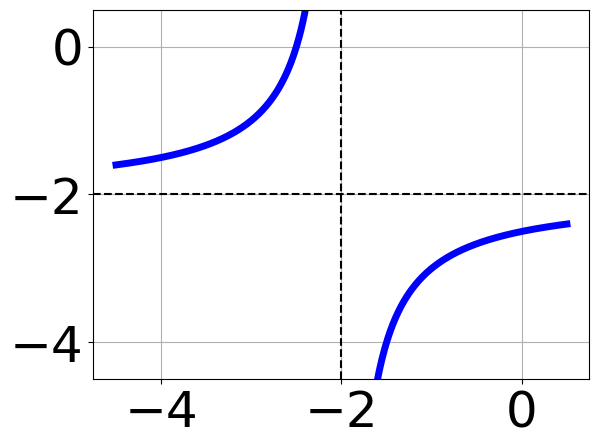
\includegraphics[width=0.3\textwidth]{../Figures/rationalEquationToGraphCopyBA.png}
    \end{center}\begin{enumerate}[label=\Alph*.]
\begin{multicols}{2}
\item 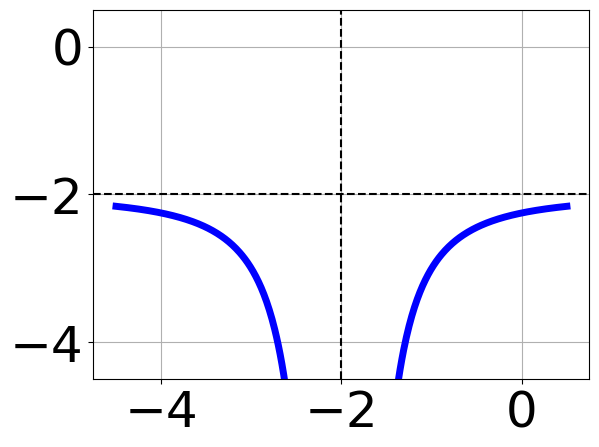
\includegraphics[width = 0.3\textwidth]{../Figures/rationalEquationToGraphCopyAA.png}
\item 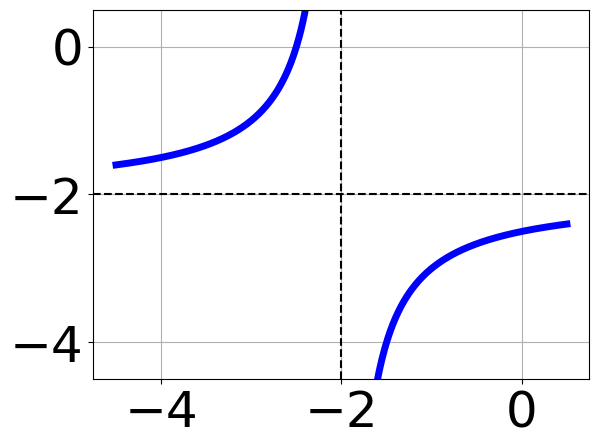
\includegraphics[width = 0.3\textwidth]{../Figures/rationalEquationToGraphCopyBA.png}
\item 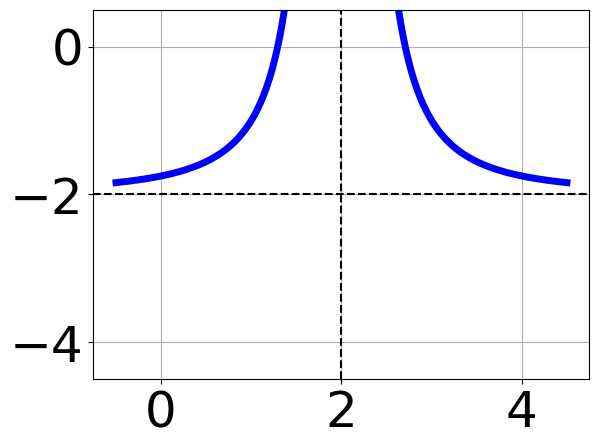
\includegraphics[width = 0.3\textwidth]{../Figures/rationalEquationToGraphCopyCA.png}
\item 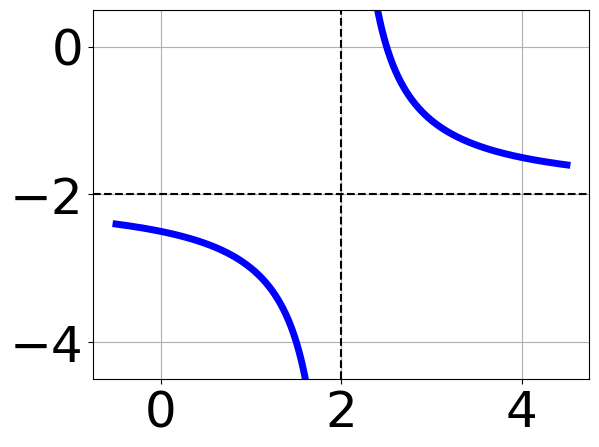
\includegraphics[width = 0.3\textwidth]{../Figures/rationalEquationToGraphCopyDA.png}
\end{multicols}\item None of the above.\end{enumerate}
\textbf{General Comment:} Remember that the general form of a basic rational equation is $ f(x) = \frac{a}{(x-h)^n} + k$, where $a$ is the leading coefficient (and in this case, we assume is either $1$ or $-1$), $n$ is the degree (in this case, either $1$ or $2$), and $(h, k)$ is the intersection of the asymptotes.
}
\litem{
Solve the rational equation below. Then, choose the interval(s) that the solution(s) belongs to.
\[ \frac{63}{54x + 27} + 1 = \frac{63}{54x + 27} \]The solution is \( \text{all solutions are invalid or lead to complex values in the equation.} \), which is option D.\begin{enumerate}[label=\Alph*.]
\item \( x \in [-0.5,0.5] \)

$x = -0.500$, which corresponds to not checking if this value leads to dividing by 0 in the original equation and thus is not a valid solution.
\item \( x_1 \in [-1.5, 0.2] \text{ and } x_2 \in [0.3,1.4] \)

$x = -0.500 \text{ and } x = 0.500$, which corresponds to getting the correct solution and believing there should be a second solution to the equation.
\item \( x_1 \in [-1.5, 0.2] \text{ and } x_2 \in [-1.4,0.1] \)

$x = -0.500 \text{ and } x = -0.500$, which corresponds to getting the correct solution and believing there should be a second solution to the equation.
\item \( \text{All solutions lead to invalid or complex values in the equation.} \)

*$x = -0.500$ leads to dividing by 0 in the original equation and thus is not a valid solution, which is the correct option.
\item \( x \in [0.3,0.8] \)

$x = 0.500$, which corresponds to not distributing the factor $54x + 27$ correctly when trying to eliminate the fraction.
\end{enumerate}

\textbf{General Comment:} Distractors are different based on the number of solutions. Remember that after solving, we need to make sure our solution does not make the original equation divide by zero!
}
\litem{
Choose the graph of the equation below.
\[ f(x) = \frac{1}{(x - 1)^2} + 3 \]The solution is the graph below, which is option E.
    \begin{center}
        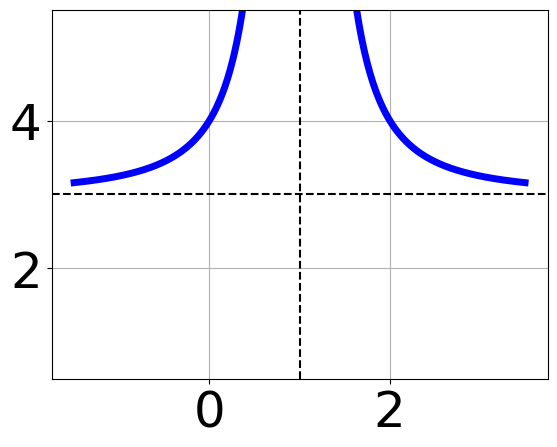
\includegraphics[width=0.3\textwidth]{../Figures/rationalEquationToGraphEA.png}
    \end{center}\begin{enumerate}[label=\Alph*.]
\begin{multicols}{2}
\item 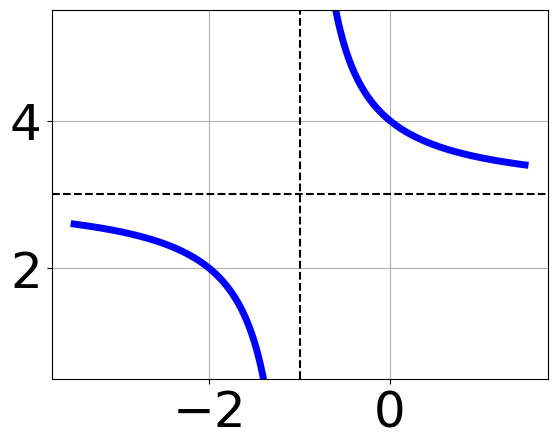
\includegraphics[width = 0.3\textwidth]{../Figures/rationalEquationToGraphAA.png}
\item 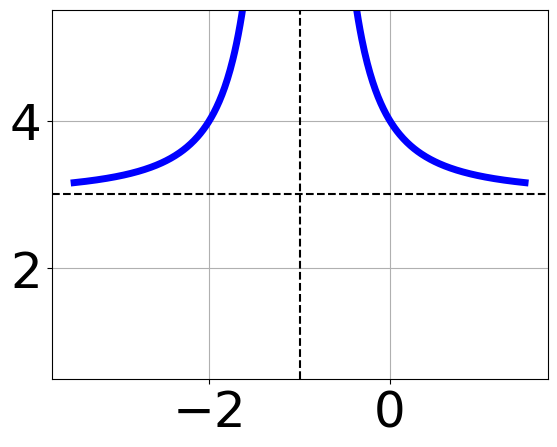
\includegraphics[width = 0.3\textwidth]{../Figures/rationalEquationToGraphBA.png}
\item 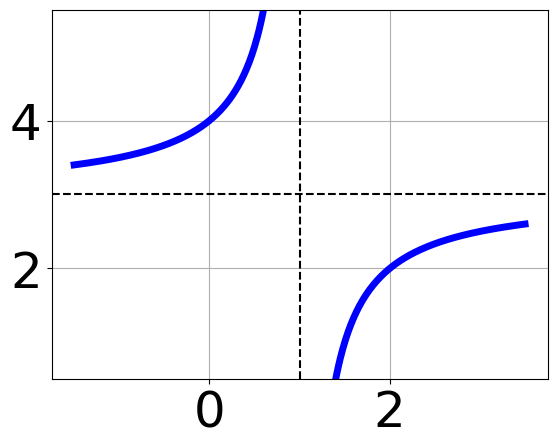
\includegraphics[width = 0.3\textwidth]{../Figures/rationalEquationToGraphCA.png}
\item 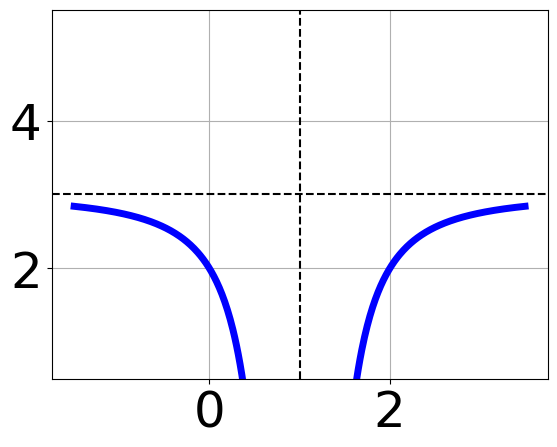
\includegraphics[width = 0.3\textwidth]{../Figures/rationalEquationToGraphDA.png}
\end{multicols}\item None of the above.\end{enumerate}
\textbf{General Comment:} Remember that the general form of a basic rational equation is $ f(x) = \frac{a}{(x-h)^n} + k$, where $a$ is the leading coefficient (and in this case, we assume is either $1$ or $-1$), $n$ is the degree (in this case, either $1$ or $2$), and $(h, k)$ is the intersection of the asymptotes.
}
\litem{
Solve the rational equation below. Then, choose the interval(s) that the solution(s) belongs to.
\[ \frac{-6}{-6x -4} + -8 = \frac{8}{48x + 32} \]The solution is \( x = -0.562 \), which is option A.\begin{enumerate}[label=\Alph*.]
\item \( x \in [-2.56,1.44] \)

* $x = -0.562$, which is the correct option.
\item \( x_1 \in [-1.3, 0.4] \text{ and } x_2 \in [0.77,1.77] \)

$x = -0.562 \text{ and } x = 0.771$, which corresponds to getting the correct solution and believing there should be a second solution to the equation.
\item \( \text{All solutions lead to invalid or complex values in the equation.} \)

This corresponds to thinking $x = -0.562$ leads to dividing by zero in the original equation, which it does not.
\item \( x_1 \in [-1.3, 0.4] \text{ and } x_2 \in [-1.38,0.62] \)

$x = -0.562 \text{ and } x = -0.375$, which corresponds to getting the correct solution and believing there should be a second solution to the equation.
\item \( x \in [0.2,1] \)

$x = 0.771$, which corresponds to not distributing the factor $-6x -4$ correctly when trying to eliminate the fraction.
\end{enumerate}

\textbf{General Comment:} Distractors are different based on the number of solutions. Remember that after solving, we need to make sure our solution does not make the original equation divide by zero!
}
\litem{
Determine the domain of the function below.
\[ f(x) = \frac{6}{15x^{2} -8 x -16} \]The solution is \( \text{All Real numbers except } x = -0.800 \text{ and } x = 1.333. \), which is option D.\begin{enumerate}[label=\Alph*.]
\item \( \text{All Real numbers except } x = a \text{ and } x = b, \text{ where } a \in [-20, -18] \text{ and } b \in [10, 15] \)

All Real numbers except $x = -20.000$ and $x = 12.000$, which corresponds to not factoring the denominator correctly.
\item \( \text{All Real numbers except } x = a, \text{ where } a \in [-0.8, 1.2] \)

All Real numbers except $x = -0.800$, which corresponds to removing only 1 value from the denominator.
\item \( \text{All Real numbers except } x = a, \text{ where } a \in [-20, -18] \)

All Real numbers except $x = -20.000$, which corresponds to removing a distractor value from the denominator.
\item \( \text{All Real numbers except } x = a \text{ and } x = b, \text{ where } a \in [-0.8, 1.2] \text{ and } b \in [0.33, 5.33] \)

All Real numbers except $x = -0.800$ and $x = 1.333$, which is the correct option.
\item \( \text{All Real numbers.} \)

This corresponds to thinking the denominator has complex roots or that rational functions have a domain of all Real numbers.
\end{enumerate}

\textbf{General Comment:} Recall that dividing by zero is not a real number. Therefore the domain is all real numbers \textbf{except} those that make the denominator 0.
}
\litem{
Solve the rational equation below. Then, choose the interval(s) that the solution(s) belongs to.
\[ \frac{-2x}{6x -7} + \frac{-3x^{2}}{24x^{2} +8 x -42} = \frac{-6}{4x + 6} \]The solution is \( \text{All solutions are invalid or lead to complex values in the equation.} \), which is option A.\begin{enumerate}[label=\Alph*.]
\item \( \text{All solutions lead to invalid or complex values in the equation.} \)

* The equation leads to solving $-5x^{2} +24 x -42=0$, which leads to complex solutions. This is the correct option.
\item \( x_1 \in [3.5, 4.4] \text{ and } x_2 \in [-1.22,3.78] \)

$x = 4.025 \text{ and } x = 0.775$, which corresponds to making the discriminant from the Quadratic Formula positive to avoid complex solutions.
\item \( x_1 \in [0.1, 1.4] \text{ and } x_2 \in [-6.5,0.5] \)

$x = 1.167 \text{ and } x = -1.500$, which corresponds to solving $6x -7 = 0$ and $4x + 6 = 0$ and treating them as solutions to the equation.
\item \( x \in [-3.7,0.3] \)

$x = -1.500$, which corresponds to solving $4x + 6 = 0$ and treating it as a solution to the equation.
\item \( x \in [0.1,1.4] \)

$x = 1.167$, which corresponds to solving $6x -7 = 0$ and treating it as a solution to the equation.
\end{enumerate}

\textbf{General Comment:} Distractors are different based on the number of solutions. Remember that after solving, we need to make sure our solution does not make the original equation divide by zero!
}
\litem{
Determine the domain of the function below.
\[ f(x) = \frac{5}{18x^{2} +15 x -25} \]The solution is \( \text{All Real numbers except } x = -1.667 \text{ and } x = 0.833. \), which is option E.\begin{enumerate}[label=\Alph*.]
\item \( \text{All Real numbers except } x = a \text{ and } x = b, \text{ where } a \in [-17, -13] \text{ and } b \in [29, 32] \)

All Real numbers except $x = -15.000$ and $x = 30.000$, which corresponds to not factoring the denominator correctly.
\item \( \text{All Real numbers.} \)

This corresponds to thinking the denominator has complex roots or that rational functions have a domain of all Real numbers.
\item \( \text{All Real numbers except } x = a, \text{ where } a \in [-3.67, -0.67] \)

All Real numbers except $x = -1.667$, which corresponds to removing only 1 value from the denominator.
\item \( \text{All Real numbers except } x = a, \text{ where } a \in [-17, -13] \)

All Real numbers except $x = -15.000$, which corresponds to removing a distractor value from the denominator.
\item \( \text{All Real numbers except } x = a \text{ and } x = b, \text{ where } a \in [-3.67, -0.67] \text{ and } b \in [0.83, 3.83] \)

All Real numbers except $x = -1.667$ and $x = 0.833$, which is the correct option.
\end{enumerate}

\textbf{General Comment:} Recall that dividing by zero is not a real number. Therefore the domain is all real numbers \textbf{except} those that make the denominator 0.
}
\litem{
Solve the rational equation below. Then, choose the interval(s) that the solution(s) belongs to.
\[ \frac{-3x}{-2x + 6} + \frac{-2x^{2}}{12x^{2} -48 x + 36} = \frac{5}{-6x + 6} \]The solution is \( \text{There are two solutions: } x = -1.142 \text{ and } x = 1.642 \), which is option E.\begin{enumerate}[label=\Alph*.]
\item \( x \in [1.34,1.87] \)


\item \( x_1 \in [-1.15, -0.96] \text{ and } x_2 \in [3,6] \)


\item \( x \in [0.46,1.62] \)


\item \( \text{All solutions lead to invalid or complex values in the equation.} \)


\item \( x_1 \in [-1.15, -0.96] \text{ and } x_2 \in [-2.36,2.64] \)

* $x = -1.142 \text{ and } x = 1.642$, which is the correct option.
\end{enumerate}

\textbf{General Comment:} Distractors are different based on the number of solutions. Remember that after solving, we need to make sure our solution does not make the original equation divide by zero!
}
\litem{
Choose the equation of the function graphed below.

\begin{center}
    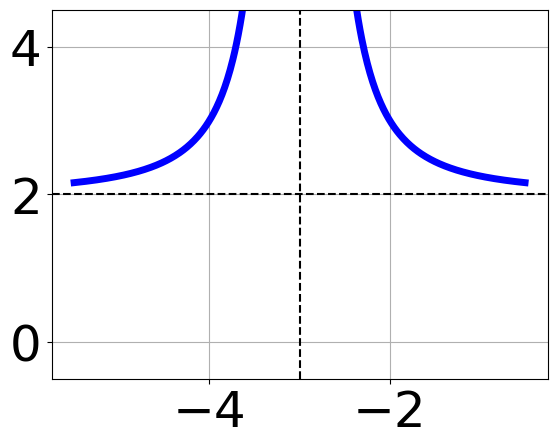
\includegraphics[width=0.5\textwidth]{../Figures/rationalGraphToEquationA.png}
\end{center}


The solution is \( \text{None of the above as it should be } f(x) = \frac{1}{(x + 3)^2} + 2 \), which is option E.\begin{enumerate}[label=\Alph*.]
\item \( f(x) = \frac{-1}{(x + 3)^2} + 2 \)

Corresponds to using the general form $f(x) = \frac{a}{(x-h)^2}+k$ and the opposite leading coefficient.
\item \( f(x) = \frac{-1}{x + 3} + 2 \)

Corresponds to thinking the graph was a shifted version of $\frac{1}{x}$, using the general form $f(x) = \frac{a}{(x-h)^2}+k$, and the opposite leading coefficient.
\item \( f(x) = \frac{1}{(x - 3)^2} + 2 \)

The $x$-value of the equation does not match the graph.
\item \( f(x) = \frac{1}{x - 3} + 2 \)

Corresponds to thinking the graph was a shifted version of $\frac{1}{x}$.
\item \( \text{None of the above} \)

None of the equation options were the correct equation.
\end{enumerate}

\textbf{General Comment:} Remember that the general form of a basic rational equation is $ f(x) = \frac{a}{(x-h)^n} + k$, where $a$ is the leading coefficient (and in this case, we assume is either $1$ or $-1$), $n$ is the degree (in this case, either $1$ or $2$), and $(h, k)$ is the intersection of the asymptotes.
}
\litem{
Choose the equation of the function graphed below.

\begin{center}
    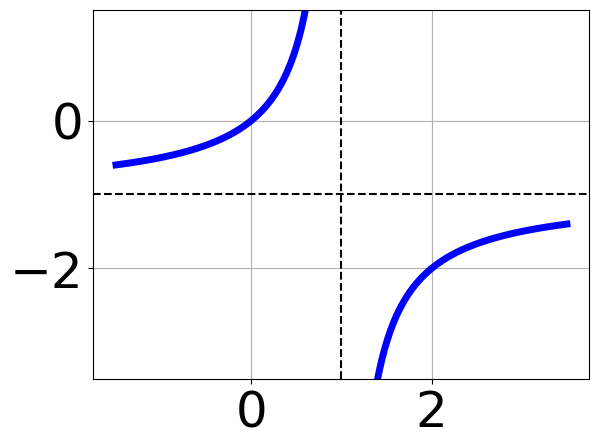
\includegraphics[width=0.5\textwidth]{../Figures/rationalGraphToEquationCopyA.png}
\end{center}


The solution is \( f(x) = \frac{-1}{x - 1} - 1 \), which is option C.\begin{enumerate}[label=\Alph*.]
\item \( f(x) = \frac{1}{x + 1} - 1 \)

Corresponds to using the general form $f(x) = \frac{a}{x+h}+k$ and the opposite leading coefficient.
\item \( f(x) = \frac{-1}{(x - 1)^2} - 1 \)

Corresponds to thinking the graph was a shifted version of $\frac{1}{x^2}$.
\item \( f(x) = \frac{-1}{x - 1} - 1 \)

This is the correct option.
\item \( f(x) = \frac{1}{(x + 1)^2} - 1 \)

Corresponds to thinking the graph was a shifted version of $\frac{1}{x^2}$, using the general form $f(x) = \frac{a}{x+h}+k$, and the opposite leading coefficient.
\item \( \text{None of the above} \)

This corresponds to believing the vertex of the graph was not correct.
\end{enumerate}

\textbf{General Comment:} Remember that the general form of a basic rational equation is $ f(x) = \frac{a}{(x-h)^n} + k$, where $a$ is the leading coefficient (and in this case, we assume is either $1$ or $-1$), $n$ is the degree (in this case, either $1$ or $2$), and $(h, k)$ is the intersection of the asymptotes.
}
\litem{
Choose the graph of the equation below.
\[ f(x) = \frac{-1}{x - 3} + 1 \]The solution is the graph below, which is option C.
    \begin{center}
        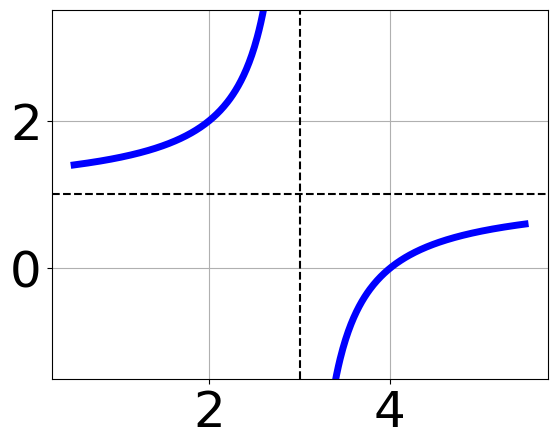
\includegraphics[width=0.3\textwidth]{../Figures/rationalEquationToGraphCopyCB.png}
    \end{center}\begin{enumerate}[label=\Alph*.]
\begin{multicols}{2}
\item 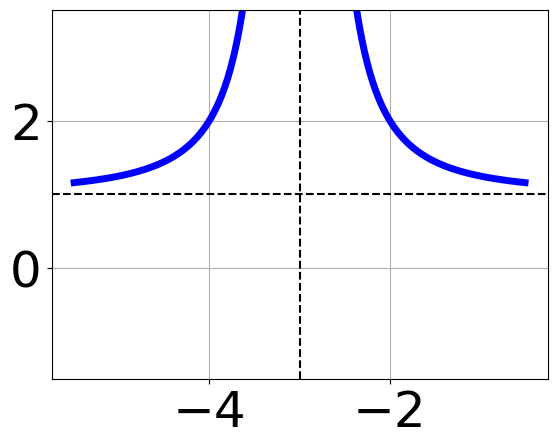
\includegraphics[width = 0.3\textwidth]{../Figures/rationalEquationToGraphCopyAB.png}
\item 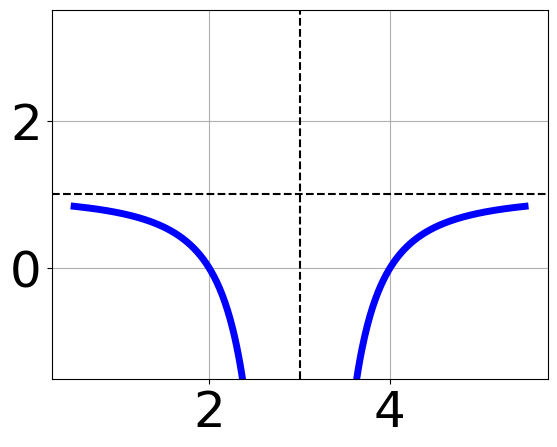
\includegraphics[width = 0.3\textwidth]{../Figures/rationalEquationToGraphCopyBB.png}
\item 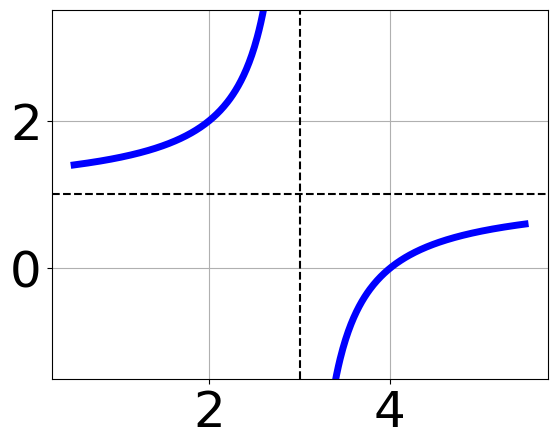
\includegraphics[width = 0.3\textwidth]{../Figures/rationalEquationToGraphCopyCB.png}
\item 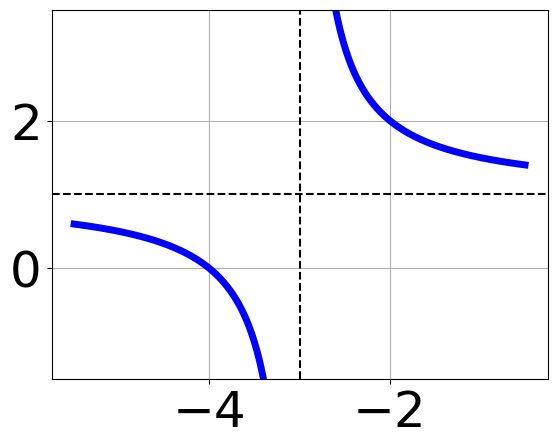
\includegraphics[width = 0.3\textwidth]{../Figures/rationalEquationToGraphCopyDB.png}
\end{multicols}\item None of the above.\end{enumerate}
\textbf{General Comment:} Remember that the general form of a basic rational equation is $ f(x) = \frac{a}{(x-h)^n} + k$, where $a$ is the leading coefficient (and in this case, we assume is either $1$ or $-1$), $n$ is the degree (in this case, either $1$ or $2$), and $(h, k)$ is the intersection of the asymptotes.
}
\litem{
Solve the rational equation below. Then, choose the interval(s) that the solution(s) belongs to.
\[ \frac{-3}{-9x + 9} + 2 = \frac{9}{81x -81} \]The solution is \( x = 0.889 \), which is option B.\begin{enumerate}[label=\Alph*.]
\item \( \text{All solutions lead to invalid or complex values in the equation.} \)

This corresponds to thinking $x = 0.889$ leads to dividing by zero in the original equation, which it does not.
\item \( x \in [0.89,1.89] \)

* $x = 0.889$, which is the correct option.
\item \( x_1 \in [-0.8, 0.5] \text{ and } x_2 \in [-1.11,2.89] \)

$x = 0.333 \text{ and } x = 0.889$, which corresponds to getting the correct solution and believing there should be a second solution to the equation.
\item \( x \in [-2.8,-0.5] \)

$x = -1.111$, which corresponds to not distributing the factor $-9x + 9$ correctly when trying to eliminate the fraction.
\item \( x_1 \in [-2.8, -0.5] \text{ and } x_2 \in [-1.11,2.89] \)

$x = -1.111 \text{ and } x = 0.889$, which corresponds to getting the correct solution and believing there should be a second solution to the equation.
\end{enumerate}

\textbf{General Comment:} Distractors are different based on the number of solutions. Remember that after solving, we need to make sure our solution does not make the original equation divide by zero!
}
\litem{
Choose the graph of the equation below.
\[ f(x) = \frac{-1}{x + 2} + 2 \]The solution is the graph below, which is option E.
    \begin{center}
        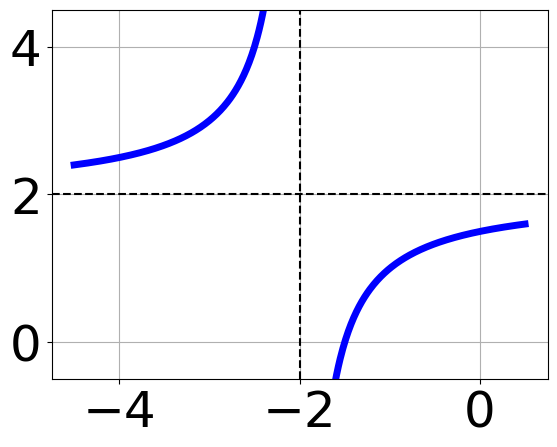
\includegraphics[width=0.3\textwidth]{../Figures/rationalEquationToGraphEB.png}
    \end{center}\begin{enumerate}[label=\Alph*.]
\begin{multicols}{2}
\item 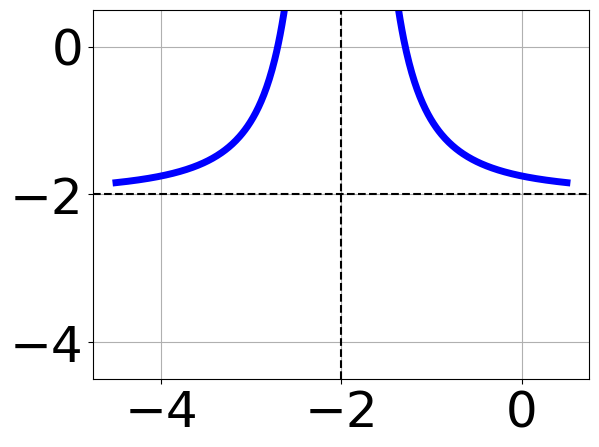
\includegraphics[width = 0.3\textwidth]{../Figures/rationalEquationToGraphAB.png}
\item 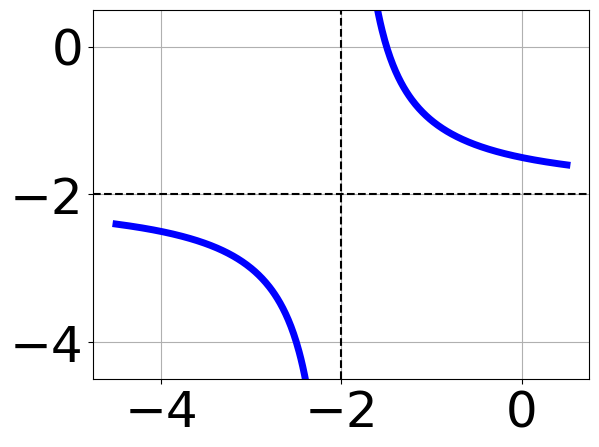
\includegraphics[width = 0.3\textwidth]{../Figures/rationalEquationToGraphBB.png}
\item 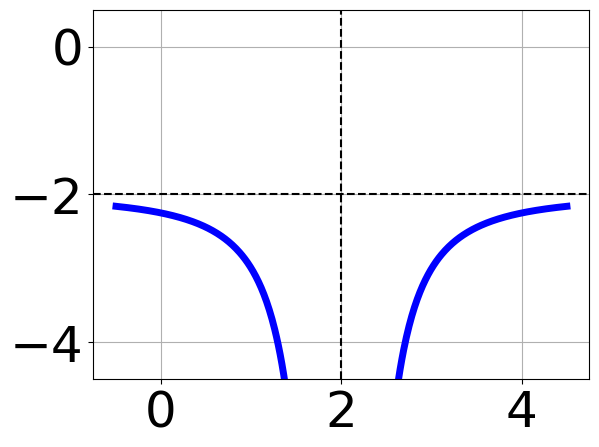
\includegraphics[width = 0.3\textwidth]{../Figures/rationalEquationToGraphCB.png}
\item 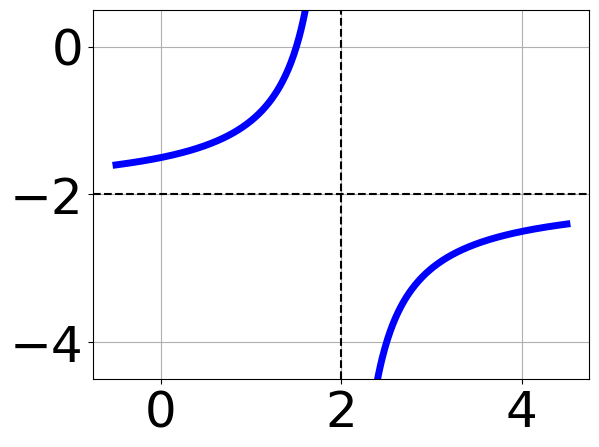
\includegraphics[width = 0.3\textwidth]{../Figures/rationalEquationToGraphDB.png}
\end{multicols}\item None of the above.\end{enumerate}
\textbf{General Comment:} Remember that the general form of a basic rational equation is $ f(x) = \frac{a}{(x-h)^n} + k$, where $a$ is the leading coefficient (and in this case, we assume is either $1$ or $-1$), $n$ is the degree (in this case, either $1$ or $2$), and $(h, k)$ is the intersection of the asymptotes.
}
\litem{
Solve the rational equation below. Then, choose the interval(s) that the solution(s) belongs to.
\[ \frac{-45}{-72x + 18} + 1 = \frac{-45}{-72x + 18} \]The solution is \( \text{all solutions are invalid or lead to complex values in the equation.} \), which is option C.\begin{enumerate}[label=\Alph*.]
\item \( x_1 \in [-0.7, -0.1] \text{ and } x_2 \in [0.25,4.25] \)

$x = -0.250 \text{ and } x = 0.250$, which corresponds to getting the correct solution and believing there should be a second solution to the equation.
\item \( x \in [-0.7,-0.1] \)

$x = -0.250$, which corresponds to not distributing the factor $-72x + 18$ correctly when trying to eliminate the fraction.
\item \( \text{All solutions lead to invalid or complex values in the equation.} \)

*$x = 0.250$ leads to dividing by 0 in the original equation and thus is not a valid solution, which is the correct option.
\item \( x \in [-0.75,1.25] \)

$x = 0.250$, which corresponds to not checking if this value leads to dividing by 0 in the original equation and thus is not a valid solution.
\item \( x_1 \in [0.1, 0.9] \text{ and } x_2 \in [0.25,4.25] \)

$x = 0.250 \text{ and } x = 0.250$, which corresponds to getting the correct solution and believing there should be a second solution to the equation.
\end{enumerate}

\textbf{General Comment:} Distractors are different based on the number of solutions. Remember that after solving, we need to make sure our solution does not make the original equation divide by zero!
}
\litem{
Determine the domain of the function below.
\[ f(x) = \frac{4}{9x^{2} -21 x + 12} \]The solution is \( \text{All Real numbers except } x = 1.000 \text{ and } x = 1.333. \), which is option B.\begin{enumerate}[label=\Alph*.]
\item \( \text{All Real numbers except } x = a, \text{ where } a \in [0.73, 1.27] \)

All Real numbers except $x = 1.000$, which corresponds to removing only 1 value from the denominator.
\item \( \text{All Real numbers except } x = a \text{ and } x = b, \text{ where } a \in [0.73, 1.27] \text{ and } b \in [1.07, 1.91] \)

All Real numbers except $x = 1.000$ and $x = 1.333$, which is the correct option.
\item \( \text{All Real numbers except } x = a, \text{ where } a \in [8.88, 9.19] \)

All Real numbers except $x = 9.000$, which corresponds to removing a distractor value from the denominator.
\item \( \text{All Real numbers.} \)

This corresponds to thinking the denominator has complex roots or that rational functions have a domain of all Real numbers.
\item \( \text{All Real numbers except } x = a \text{ and } x = b, \text{ where } a \in [8.88, 9.19] \text{ and } b \in [11.76, 12.03] \)

All Real numbers except $x = 9.000$ and $x = 12.000$, which corresponds to not factoring the denominator correctly.
\end{enumerate}

\textbf{General Comment:} Recall that dividing by zero is not a real number. Therefore the domain is all real numbers \textbf{except} those that make the denominator 0.
}
\litem{
Solve the rational equation below. Then, choose the interval(s) that the solution(s) belongs to.
\[ \frac{-6x}{3x + 6} + \frac{-5x^{2}}{21x^{2} +57 x + 30} = \frac{-5}{7x + 5} \]The solution is \( \text{There are two solutions: } x = 0.655 \text{ and } x = -0.974 \), which is option A.\begin{enumerate}[label=\Alph*.]
\item \( x_1 \in [0.48, 0.9] \text{ and } x_2 \in [-1.97,4.03] \)

* $x = 0.655 \text{ and } x = -0.974$, which is the correct option.
\item \( \text{All solutions lead to invalid or complex values in the equation.} \)


\item \( x \in [-1.35,-0.83] \)


\item \( x \in [-0.88,-0.71] \)


\item \( x_1 \in [0.48, 0.9] \text{ and } x_2 \in [-5,-1] \)


\end{enumerate}

\textbf{General Comment:} Distractors are different based on the number of solutions. Remember that after solving, we need to make sure our solution does not make the original equation divide by zero!
}
\litem{
Determine the domain of the function below.
\[ f(x) = \frac{4}{18x^{2} +21 x -15} \]The solution is \( \text{All Real numbers except } x = -1.667 \text{ and } x = 0.500. \), which is option C.\begin{enumerate}[label=\Alph*.]
\item \( \text{All Real numbers.} \)

This corresponds to thinking the denominator has complex roots or that rational functions have a domain of all Real numbers.
\item \( \text{All Real numbers except } x = a, \text{ where } a \in [-4.67, -0.67] \)

All Real numbers except $x = -1.667$, which corresponds to removing only 1 value from the denominator.
\item \( \text{All Real numbers except } x = a \text{ and } x = b, \text{ where } a \in [-4.67, -0.67] \text{ and } b \in [-0.5, 1.5] \)

All Real numbers except $x = -1.667$ and $x = 0.500$, which is the correct option.
\item \( \text{All Real numbers except } x = a, \text{ where } a \in [-17, -12] \)

All Real numbers except $x = -15.000$, which corresponds to removing a distractor value from the denominator.
\item \( \text{All Real numbers except } x = a \text{ and } x = b, \text{ where } a \in [-17, -12] \text{ and } b \in [15, 20] \)

All Real numbers except $x = -15.000$ and $x = 18.000$, which corresponds to not factoring the denominator correctly.
\end{enumerate}

\textbf{General Comment:} Recall that dividing by zero is not a real number. Therefore the domain is all real numbers \textbf{except} those that make the denominator 0.
}
\litem{
Solve the rational equation below. Then, choose the interval(s) that the solution(s) belongs to.
\[ \frac{-6x}{-6x -4} + \frac{-7x^{2}}{-30x^{2} -2 x + 12} = \frac{3}{5x -3} \]The solution is \( \text{There are two solutions: } x = -0.263 \text{ and } x = 1.235 \), which is option D.\begin{enumerate}[label=\Alph*.]
\item \( \text{All solutions lead to invalid or complex values in the equation.} \)


\item \( x \in [1.09,1.68] \)


\item \( x_1 \in [-1.53, -0.16] \text{ and } x_2 \in [-1.8,-0.3] \)


\item \( x_1 \in [-1.53, -0.16] \text{ and } x_2 \in [0.7,1.5] \)

* $x = -0.263 \text{ and } x = 1.235$, which is the correct option.
\item \( x \in [0.46,1.06] \)


\end{enumerate}

\textbf{General Comment:} Distractors are different based on the number of solutions. Remember that after solving, we need to make sure our solution does not make the original equation divide by zero!
}
\litem{
Choose the equation of the function graphed below.

\begin{center}
    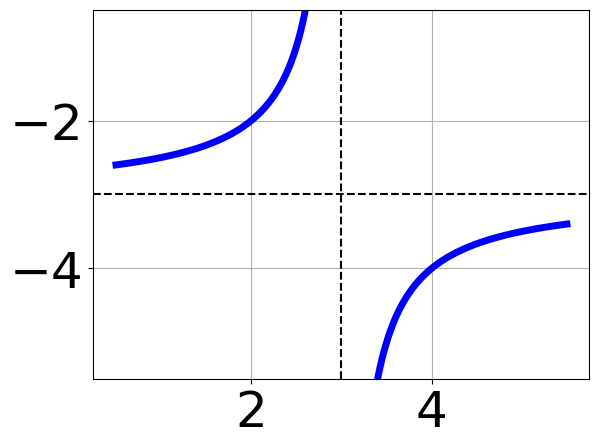
\includegraphics[width=0.5\textwidth]{../Figures/rationalGraphToEquationB.png}
\end{center}


The solution is \( f(x) = \frac{-1}{x - 3} - 3 \), which is option C.\begin{enumerate}[label=\Alph*.]
\item \( f(x) = \frac{1}{(x + 3)^2} - 3 \)

Corresponds to thinking the graph was a shifted version of $\frac{1}{x^2}$, using the general form $f(x) = \frac{a}{x+h}+k$, and the opposite leading coefficient.
\item \( f(x) = \frac{1}{x + 3} - 3 \)

Corresponds to using the general form $f(x) = \frac{a}{x+h}+k$ and the opposite leading coefficient.
\item \( f(x) = \frac{-1}{x - 3} - 3 \)

This is the correct option.
\item \( f(x) = \frac{-1}{(x - 3)^2} - 3 \)

Corresponds to thinking the graph was a shifted version of $\frac{1}{x^2}$.
\item \( \text{None of the above} \)

This corresponds to believing the vertex of the graph was not correct.
\end{enumerate}

\textbf{General Comment:} Remember that the general form of a basic rational equation is $ f(x) = \frac{a}{(x-h)^n} + k$, where $a$ is the leading coefficient (and in this case, we assume is either $1$ or $-1$), $n$ is the degree (in this case, either $1$ or $2$), and $(h, k)$ is the intersection of the asymptotes.
}
\litem{
Choose the equation of the function graphed below.

\begin{center}
    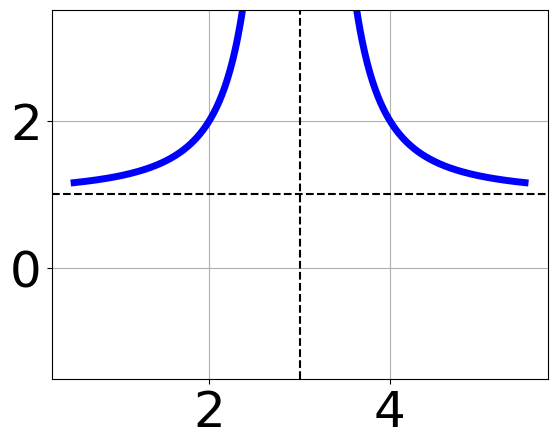
\includegraphics[width=0.5\textwidth]{../Figures/rationalGraphToEquationCopyB.png}
\end{center}


The solution is \( f(x) = \frac{1}{(x - 3)^2} + 1 \), which is option D.\begin{enumerate}[label=\Alph*.]
\item \( f(x) = \frac{1}{x - 3} + 1 \)

Corresponds to thinking the graph was a shifted version of $\frac{1}{x}$.
\item \( f(x) = \frac{-1}{(x + 3)^2} + 1 \)

Corresponds to using the general form $f(x) = \frac{a}{(x+h)^2}+k$ and the opposite leading coefficient.
\item \( f(x) = \frac{-1}{x + 3} + 1 \)

Corresponds to thinking the graph was a shifted version of $\frac{1}{x}$, using the general form $f(x) = \frac{a}{(x+h)^2}+k$, and the opposite leading coefficient.
\item \( f(x) = \frac{1}{(x - 3)^2} + 1 \)

This is the correct option.
\item \( \text{None of the above} \)

This corresponds to believing the vertex of the graph was not correct.
\end{enumerate}

\textbf{General Comment:} Remember that the general form of a basic rational equation is $ f(x) = \frac{a}{(x-h)^n} + k$, where $a$ is the leading coefficient (and in this case, we assume is either $1$ or $-1$), $n$ is the degree (in this case, either $1$ or $2$), and $(h, k)$ is the intersection of the asymptotes.
}
\litem{
Choose the graph of the equation below.
\[ f(x) = \frac{-1}{x + 3} - 1 \]The solution is the graph below, which is option A.
    \begin{center}
        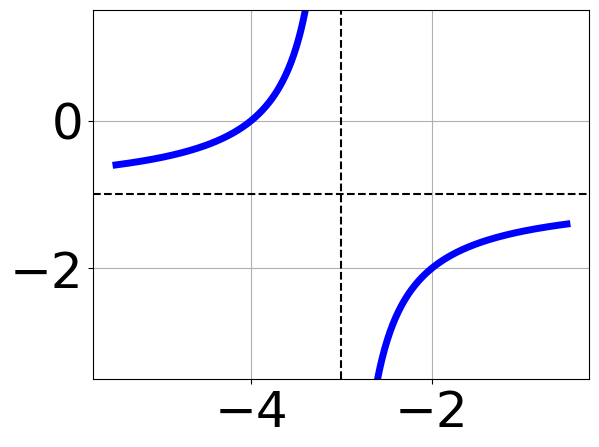
\includegraphics[width=0.3\textwidth]{../Figures/rationalEquationToGraphCopyAC.png}
    \end{center}\begin{enumerate}[label=\Alph*.]
\begin{multicols}{2}
\item 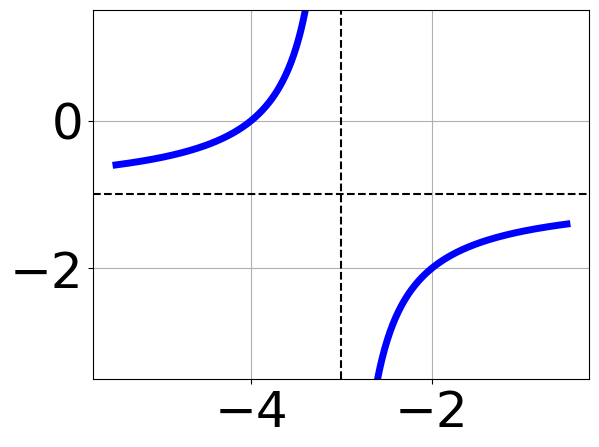
\includegraphics[width = 0.3\textwidth]{../Figures/rationalEquationToGraphCopyAC.png}
\item 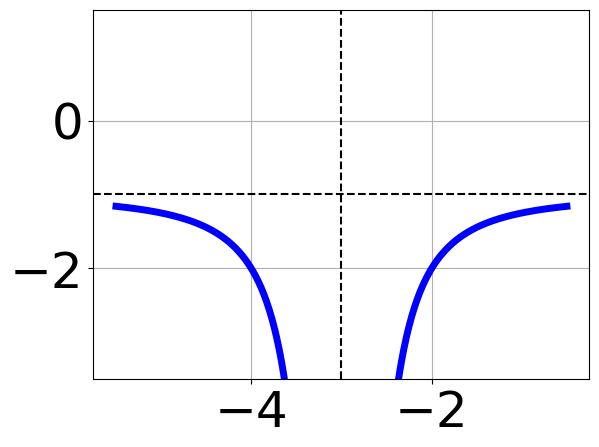
\includegraphics[width = 0.3\textwidth]{../Figures/rationalEquationToGraphCopyBC.png}
\item 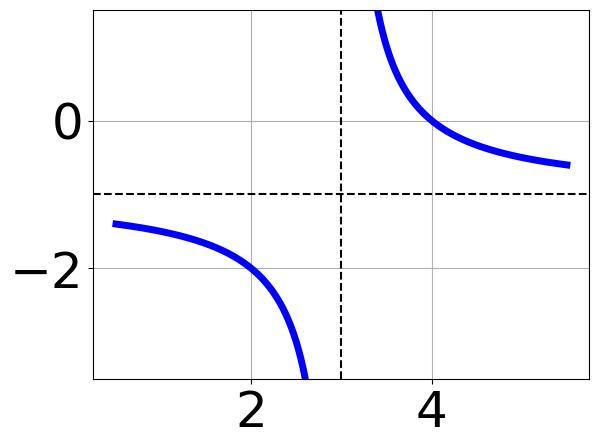
\includegraphics[width = 0.3\textwidth]{../Figures/rationalEquationToGraphCopyCC.png}
\item 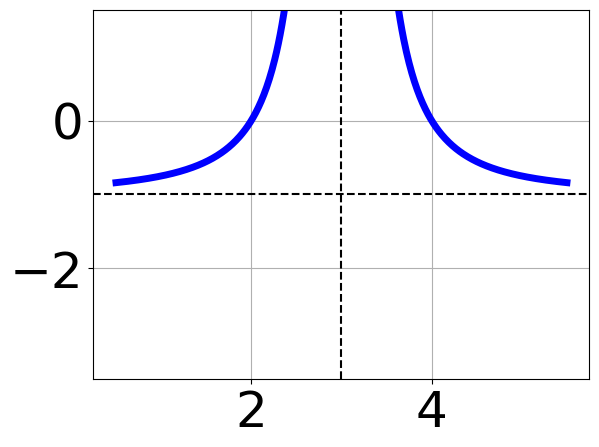
\includegraphics[width = 0.3\textwidth]{../Figures/rationalEquationToGraphCopyDC.png}
\end{multicols}\item None of the above.\end{enumerate}
\textbf{General Comment:} Remember that the general form of a basic rational equation is $ f(x) = \frac{a}{(x-h)^n} + k$, where $a$ is the leading coefficient (and in this case, we assume is either $1$ or $-1$), $n$ is the degree (in this case, either $1$ or $2$), and $(h, k)$ is the intersection of the asymptotes.
}
\litem{
Solve the rational equation below. Then, choose the interval(s) that the solution(s) belongs to.
\[ \frac{56}{70x -70} + 1 = \frac{56}{70x -70} \]The solution is \( \text{all solutions are invalid or lead to complex values in the equation.} \), which is option B.\begin{enumerate}[label=\Alph*.]
\item \( x \in [-2,0] \)

$x = -1.000$, which corresponds to not distributing the factor $70x -70$ correctly when trying to eliminate the fraction.
\item \( \text{All solutions lead to invalid or complex values in the equation.} \)

*$x = 1.000$ leads to dividing by 0 in the original equation and thus is not a valid solution, which is the correct option.
\item \( x_1 \in [-2, 0] \text{ and } x_2 \in [-1,3] \)

$x = -1.000 \text{ and } x = 1.000$, which corresponds to getting the correct solution and believing there should be a second solution to the equation.
\item \( x_1 \in [0, 2] \text{ and } x_2 \in [-1,3] \)

$x = 1.000 \text{ and } x = 1.000$, which corresponds to getting the correct solution and believing there should be a second solution to the equation.
\item \( x \in [1.0,2.0] \)

$x = 1.000$, which corresponds to not checking if this value leads to dividing by 0 in the original equation and thus is not a valid solution.
\end{enumerate}

\textbf{General Comment:} Distractors are different based on the number of solutions. Remember that after solving, we need to make sure our solution does not make the original equation divide by zero!
}
\litem{
Choose the graph of the equation below.
\[ f(x) = \frac{1}{x + 1} - 2 \]The solution is the graph below, which is option C.
    \begin{center}
        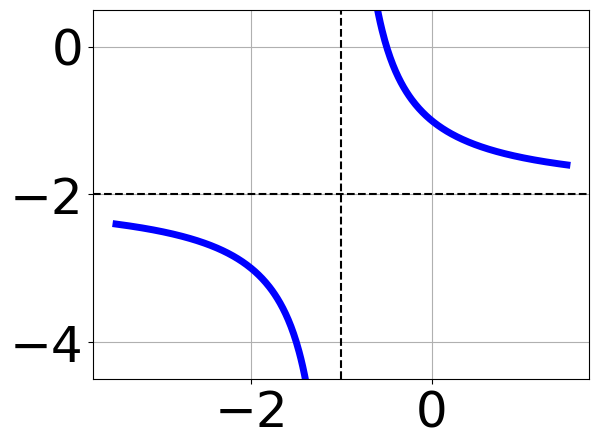
\includegraphics[width=0.3\textwidth]{../Figures/rationalEquationToGraphCC.png}
    \end{center}\begin{enumerate}[label=\Alph*.]
\begin{multicols}{2}
\item 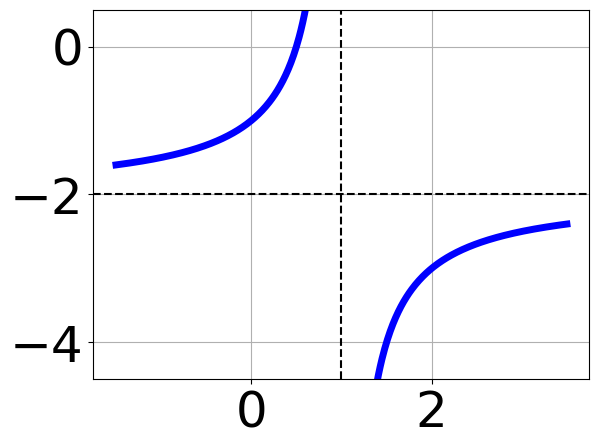
\includegraphics[width = 0.3\textwidth]{../Figures/rationalEquationToGraphAC.png}
\item 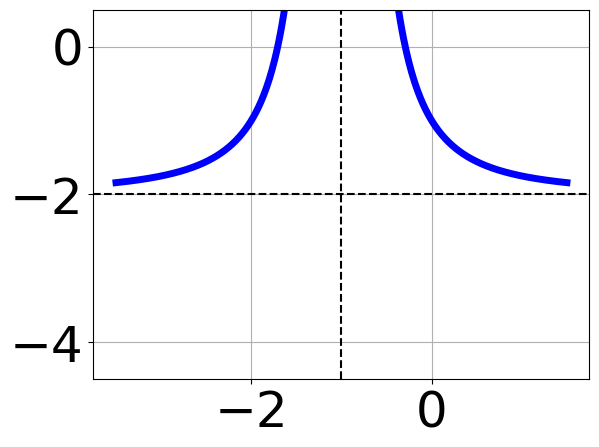
\includegraphics[width = 0.3\textwidth]{../Figures/rationalEquationToGraphBC.png}
\item 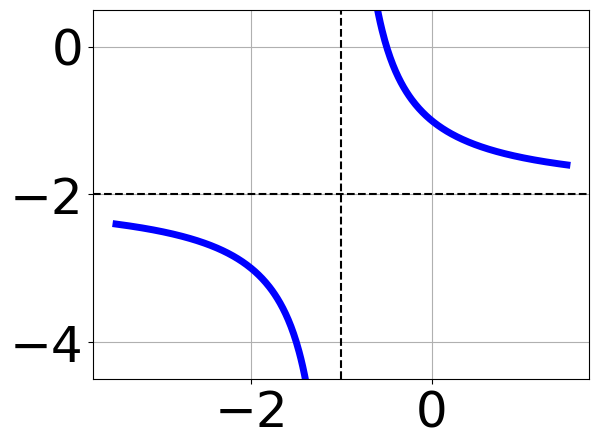
\includegraphics[width = 0.3\textwidth]{../Figures/rationalEquationToGraphCC.png}
\item 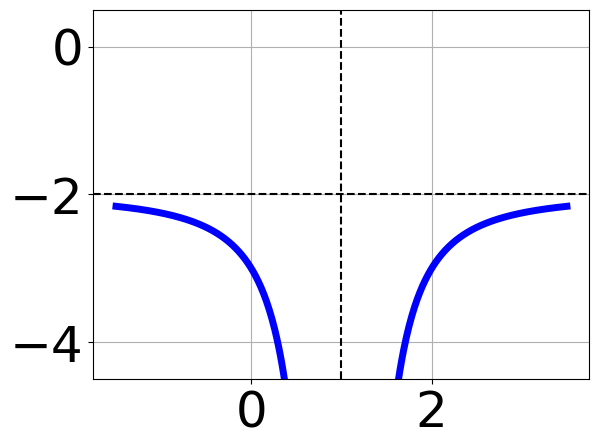
\includegraphics[width = 0.3\textwidth]{../Figures/rationalEquationToGraphDC.png}
\end{multicols}\item None of the above.\end{enumerate}
\textbf{General Comment:} Remember that the general form of a basic rational equation is $ f(x) = \frac{a}{(x-h)^n} + k$, where $a$ is the leading coefficient (and in this case, we assume is either $1$ or $-1$), $n$ is the degree (in this case, either $1$ or $2$), and $(h, k)$ is the intersection of the asymptotes.
}
\litem{
Solve the rational equation below. Then, choose the interval(s) that the solution(s) belongs to.
\[ \frac{2}{4x + 4} + -8 = \frac{5}{24x + 24} \]The solution is \( x = -0.964 \), which is option D.\begin{enumerate}[label=\Alph*.]
\item \( x_1 \in [-1.09, -0.57] \text{ and } x_2 \in [-0.96,5.04] \)

$x = -0.964 \text{ and } x = 1.036$, which corresponds to getting the correct solution and believing there should be a second solution to the equation.
\item \( \text{All solutions lead to invalid or complex values in the equation.} \)

This corresponds to thinking $x = -0.964$ leads to dividing by zero in the original equation, which it does not.
\item \( x_1 \in [-1.15, -1.01] \text{ and } x_2 \in [-1.96,0.04] \)

$x = -1.094 \text{ and } x = -0.964$, which corresponds to getting the correct solution and believing there should be a second solution to the equation.
\item \( x \in [-1.96,0.04] \)

* $x = -0.964$, which is the correct option.
\item \( x \in [0.38,1.12] \)

$x = 1.036$, which corresponds to not distributing the factor $4x + 4$ correctly when trying to eliminate the fraction.
\end{enumerate}

\textbf{General Comment:} Distractors are different based on the number of solutions. Remember that after solving, we need to make sure our solution does not make the original equation divide by zero!
}
\litem{
Determine the domain of the function below.
\[ f(x) = \frac{6}{30x^{2} -39 x + 12} \]The solution is \( \text{All Real numbers except } x = 0.500 \text{ and } x = 0.800. \), which is option B.\begin{enumerate}[label=\Alph*.]
\item \( \text{All Real numbers except } x = a, \text{ where } a \in [17.92, 18.17] \)

All Real numbers except $x = 18.000$, which corresponds to removing a distractor value from the denominator.
\item \( \text{All Real numbers except } x = a \text{ and } x = b, \text{ where } a \in [0.29, 0.5] \text{ and } b \in [0.56, 0.94] \)

All Real numbers except $x = 0.500$ and $x = 0.800$, which is the correct option.
\item \( \text{All Real numbers except } x = a, \text{ where } a \in [0.29, 0.5] \)

All Real numbers except $x = 0.500$, which corresponds to removing only 1 value from the denominator.
\item \( \text{All Real numbers.} \)

This corresponds to thinking the denominator has complex roots or that rational functions have a domain of all Real numbers.
\item \( \text{All Real numbers except } x = a \text{ and } x = b, \text{ where } a \in [17.92, 18.17] \text{ and } b \in [19.87, 20.04] \)

All Real numbers except $x = 18.000$ and $x = 20.000$, which corresponds to not factoring the denominator correctly.
\end{enumerate}

\textbf{General Comment:} Recall that dividing by zero is not a real number. Therefore the domain is all real numbers \textbf{except} those that make the denominator 0.
}
\litem{
Solve the rational equation below. Then, choose the interval(s) that the solution(s) belongs to.
\[ \frac{2x}{-5x -7} + \frac{-6x^{2}}{35x^{2} +84 x + 49} = \frac{-3}{-7x -7} \]The solution is \( \text{All solutions are invalid or lead to complex values in the equation.} \), which is option A.\begin{enumerate}[label=\Alph*.]
\item \( \text{All solutions lead to invalid or complex values in the equation.} \)

* The equation leads to solving $-8x^{2} -29 x -21=0$, which leads to complex solutions. This is the correct option.
\item \( x_1 \in [-1.32, -0.99] \text{ and } x_2 \in [-3.06,-1.77] \)

$x = -1.000 \text{ and } x = -2.625$, which corresponds to making the discriminant from the Quadratic Formula positive to avoid complex solutions.
\item \( x_1 \in [-1.85, -1.34] \text{ and } x_2 \in [-2.03,-0.18] \)

$x = -1.400 \text{ and } x = -1.000$, which corresponds to solving $-5x -7 = 0$ and $-7x -7 = 0$ and treating them as solutions to the equation.
\item \( x \in [-1.85,-1.34] \)

$x = -1.400$, which corresponds to solving $-5x -7 = 0$ and treating it as a solution to the equation.
\item \( x \in [-1.32,-0.99] \)

$x = -1.000$, which corresponds to solving $-7x -7 = 0$ and treating it as a solution to the equation.
\end{enumerate}

\textbf{General Comment:} Distractors are different based on the number of solutions. Remember that after solving, we need to make sure our solution does not make the original equation divide by zero!
}
\litem{
Determine the domain of the function below.
\[ f(x) = \frac{5}{12x^{2} -25 x + 12} \]The solution is \( \text{All Real numbers except } x = 0.750 \text{ and } x = 1.333. \), which is option A.\begin{enumerate}[label=\Alph*.]
\item \( \text{All Real numbers except } x = a \text{ and } x = b, \text{ where } a \in [-0.52, 0.88] \text{ and } b \in [0.86, 1.81] \)

All Real numbers except $x = 0.750$ and $x = 1.333$, which is the correct option.
\item \( \text{All Real numbers except } x = a \text{ and } x = b, \text{ where } a \in [10.75, 13.23] \text{ and } b \in [10.75, 13.23] \)

All Real numbers except $x = 12.000$ and $x = 12.000$, which corresponds to not factoring the denominator correctly.
\item \( \text{All Real numbers.} \)

This corresponds to thinking the denominator has complex roots or that rational functions have a domain of all Real numbers.
\item \( \text{All Real numbers except } x = a, \text{ where } a \in [10.75, 13.23] \)

All Real numbers except $x = 12.000$, which corresponds to removing a distractor value from the denominator.
\item \( \text{All Real numbers except } x = a, \text{ where } a \in [-0.52, 0.88] \)

All Real numbers except $x = 0.750$, which corresponds to removing only 1 value from the denominator.
\end{enumerate}

\textbf{General Comment:} Recall that dividing by zero is not a real number. Therefore the domain is all real numbers \textbf{except} those that make the denominator 0.
}
\litem{
Solve the rational equation below. Then, choose the interval(s) that the solution(s) belongs to.
\[ \frac{-5x}{-5x -5} + \frac{-3x^{2}}{-10x^{2} +25 x + 35} = \frac{-7}{2x -7} \]The solution is \( \text{All solutions are invalid or lead to complex values in the equation.} \), which is option C.\begin{enumerate}[label=\Alph*.]
\item \( x_1 \in [-2.01, -0.31] \text{ and } x_2 \in [1.5,5.5] \)

$x = -1.000 \text{ and } x = 3.500$, which corresponds to solving $-5x -5 = 0$ and $2x -7 = 0$ and treating them as solutions to the equation.
\item \( x \in [3.05,3.68] \)

$x = 3.500$, which corresponds to solving $2x -7 = 0$ and treating it as a solution to the equation.
\item \( \text{All solutions lead to invalid or complex values in the equation.} \)

* The equation leads to solving $-7x^{2} -35=0$, which leads to complex solutions. This is the correct option.
\item \( x \in [-2.01,-0.31] \)

$x = -1.000$, which corresponds to solving $-5x -5 = 0$ and treating it as a solution to the equation.
\item \( x_1 \in [1.91, 2.47] \text{ and } x_2 \in [-3.24,-0.24] \)

$x = 2.236 \text{ and } x = -2.236$, which corresponds to making the discriminant from the Quadratic Formula positive to avoid complex solutions.
\end{enumerate}

\textbf{General Comment:} Distractors are different based on the number of solutions. Remember that after solving, we need to make sure our solution does not make the original equation divide by zero!
}
\litem{
Choose the equation of the function graphed below.

\begin{center}
    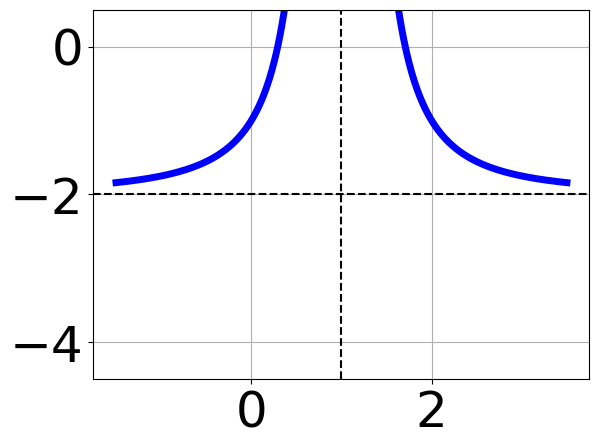
\includegraphics[width=0.5\textwidth]{../Figures/rationalGraphToEquationC.png}
\end{center}


The solution is \( \text{None of the above as it should be } f(x) = \frac{1}{(x - 1)^2} - 2 \), which is option E.\begin{enumerate}[label=\Alph*.]
\item \( f(x) = \frac{-1}{x + 1} + 2 \)

Corresponds to thinking the graph was a shifted version of $\frac{1}{x}$, using the general form $f(x) = \frac{a}{(x+h)^2}+k$, the opposite leading coefficient, AND not noticing the $y$-value was wrong.
\item \( f(x) = \frac{1}{x - 1} + 2 \)

Corresponds to thinking the graph was a shifted version of $\frac{1}{x}$ AND not noticing the $y$-value was wrong.
\item \( f(x) = \frac{1}{(x - 1)^2} + 2 \)

The $y$-value of the equation does not match the graph.
\item \( f(x) = \frac{-1}{(x + 1)^2} + 2 \)

Corresponds to using the general form $f(x) = \frac{a}{(x+h)^2}+k$, the opposite leading coefficient, AND not noticing the $y$-value was wrong.
\item \( \text{None of the above} \)

None of the equation options were the correct equation.
\end{enumerate}

\textbf{General Comment:} Remember that the general form of a basic rational equation is $ f(x) = \frac{a}{(x-h)^n} + k$, where $a$ is the leading coefficient (and in this case, we assume is either $1$ or $-1$), $n$ is the degree (in this case, either $1$ or $2$), and $(h, k)$ is the intersection of the asymptotes.
}
\litem{
Choose the equation of the function graphed below.

\begin{center}
    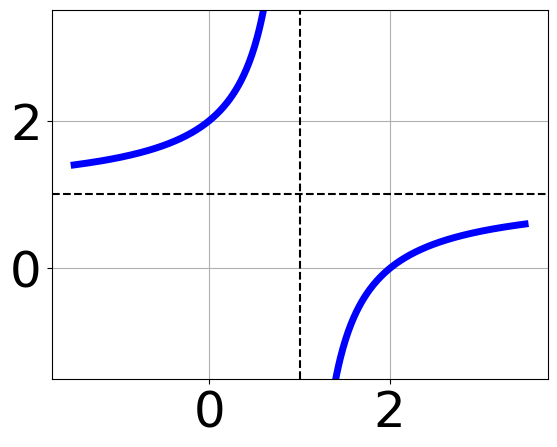
\includegraphics[width=0.5\textwidth]{../Figures/rationalGraphToEquationCopyC.png}
\end{center}


The solution is \( f(x) = \frac{-1}{x - 1} + 1 \), which is option A.\begin{enumerate}[label=\Alph*.]
\item \( f(x) = \frac{-1}{x - 1} + 1 \)

This is the correct option.
\item \( f(x) = \frac{-1}{(x - 1)^2} + 1 \)

Corresponds to thinking the graph was a shifted version of $\frac{1}{x^2}$.
\item \( f(x) = \frac{1}{x + 1} + 1 \)

Corresponds to using the general form $f(x) = \frac{a}{x+h}+k$ and the opposite leading coefficient.
\item \( f(x) = \frac{1}{(x + 1)^2} + 1 \)

Corresponds to thinking the graph was a shifted version of $\frac{1}{x^2}$, using the general form $f(x) = \frac{a}{x+h}+k$, and the opposite leading coefficient.
\item \( \text{None of the above} \)

This corresponds to believing the vertex of the graph was not correct.
\end{enumerate}

\textbf{General Comment:} Remember that the general form of a basic rational equation is $ f(x) = \frac{a}{(x-h)^n} + k$, where $a$ is the leading coefficient (and in this case, we assume is either $1$ or $-1$), $n$ is the degree (in this case, either $1$ or $2$), and $(h, k)$ is the intersection of the asymptotes.
}
\end{enumerate}

\end{document}